\documentclass{article}



\usepackage{fullpage}
\usepackage{nopageno}
\usepackage{amsmath}
\usepackage{amsfonts}
\usepackage{graphicx}
\usepackage{framed}
\usepackage{xcolor}

\definecolor{dark_red}{rgb}{0.5,0.0,0.0}
\definecolor{dark_green}{rgb}{0.0,0.5,0.0}
\definecolor{dark_blue}{rgb}{0.0,0.0,0.5}

\newcommand{\dr}[1]{\textcolor{dark_red}{#1}}
\newcommand{\dg}[1]{\textcolor{dark_green}{#1}}
\newcommand{\db}[1]{\textcolor{dark_blue}{#1}}


\begin{document}

\section{Graphs of trigonometric functions}

\begin{tabular}{cc}
\parbox{0.5\textwidth}{
\includegraphics[width = 0.5\textwidth]{cos_and_sin.png} \\
dark red \(= \cos\theta\); ~~~ light red \(= \sin\theta\)
} & \parbox{0.5\textwidth}{
\includegraphics[width = 0.5\textwidth]{tan_and_sec.png} \\
dark green \(= \tan\theta\); ~~~ light green \(= \sec\theta\)
} \\ 
\parbox{0.5\textwidth}{
\includegraphics[width = 0.5\textwidth]{cot_and_csc.png} \\
dark blue \(= \cot\theta\); ~~~ light blue \(= \csc\theta\)
} & 
\end{tabular}



\pagebreak

\section{Solving Right-triangles}

Given a right triangle where a single side is known, and one of the non-right angles is known (referred to henceforth as the {\bf named angle}), the process of finding the lengths of the other two sides is: 

\begin{tabular}{cc}
\parbox{0.5\textwidth}{
\begin{itemize}
\item If the hypotenuse \(\dr{h}\) is known, 
	\begin{itemize}
	\item The adjacent \(a = \dr{h\cos\theta}\)
	\item The opposite \(o = \dr{h\sin\theta}\)
	\end{itemize}
\item If the adjacent \(\dg{a}\) is known, 
	\begin{itemize}
	\item The opposite \(o = \dg{a\tan\theta}\)
	\item The hypotenuse \(h = \dg{a\sec\theta}\)
	\end{itemize}
\item If the opposite \(\db{o}\) is known, 
	\begin{itemize}
	\item The adjacent \(a = \db{o\cot\theta}\)
	\item The hypotenuse \(h = \db{o\csc\theta}\)
	\end{itemize}
\end{itemize}
} & \parbox{0.3\textwidth}{
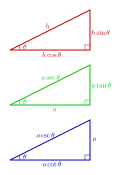
\includegraphics[width = 0.3\textwidth]{3_triangles_non_unit}
}
\end{tabular}

\textbf{Examples:}
\begin{itemize}
\item If the hypotenuse is \(h = 56.7\text{m}\), and the named angle is \(\theta = 20^\circ\), then the adjacent is \(a = h\cos\theta = (56.7\text{m})\cos(20^\circ) \approx 53.2806\text{m}\), and the opposite is \(o = h\sin\theta = (56.7\text{m})\sin(20^\circ) \approx 19.3925\text{m}\). 
%%%%%%%%%%%%%%%%
\item If the adjacent is \(a = 7.0 \times 10^4\text{m}\), and the named angle is \(\theta = 58.4^\circ\), then the opposite is \(o = a\tan\theta = (7.0 \times 10^4\text{m})\tan(58.4^\circ) \approx 1.13783 \times 10^5\text{m}\), and the hypotenuse is \(h = a\sec\theta = (7.0 \times 10^4\text{m})/\cos(58.4^\circ) \approx 1.33591 \times 10^5\text{m}\). 
%%%%%%%%%%%%%%%%
\item If the opposite is \(o = 2.14 \times 10^{-10}\text{m}\), and the named angle is \(\theta = 64.1^\circ\), then the adjacent is \(a = o\cot\theta = (2.14 \times 10^{-10}\text{m})/\tan(64.1^\circ) \approx 1.03913 \times 10^{-10}\text{m}\), and the hypotenuse is \(h = o\csc\theta = (2.14 \times 10^{-10}\text{m})/\sin(64.1^\circ) \approx 2.37895 \times 10^{-10}\text{m}\)
\end{itemize}

\begin{tabular}{cc}
\parbox{0.6\textwidth}{
In the image to the right, \(\alpha = 35^\circ\), \(\beta = 65^\circ\), \(\gamma = 40^\circ\), \(\delta = 60^\circ\), \(\epsilon = 70^\circ\), and \(\theta = 10^\circ\). \\ ~~ \\
\begin{itemize}
\item \(a = 1 \cdot \cos\alpha = \cos 35^\circ \approx 0.819152\)
\item \(b = a \cos\beta = \cos 35^\circ \cos 65^\circ \approx 0.346189\)
\item \(c = a \sin\beta = \cos 35^\circ \sin 65^\circ \approx 0.742404\)
\item \(d = c\tan\gamma = \cos 35^\circ \sin 65^\circ \tan 40^\circ \approx 0.622951\)
\item \(e = c\sec\gamma = \cos 35^\circ \sin 65^\circ \sec 40^\circ \approx 0.969139\)
\item \(f = 1 \cdot \sin\alpha = \sin 35^\circ \approx 0.573576\)
\item \(g = f\cot\delta = \sin 35^\circ \cot 60^\circ \approx 0.331155\)
\item \(h = f\csc\delta = \sin 35^\circ \csc 60^\circ \approx 0.662309\)
\item \(i = 1 \cdot \cot\epsilon = \cot 70^\circ \approx 0.363970\)
\item \(j = 1 \cdot \csc\epsilon = \csc 70^\circ \approx 1.06418\)
\item \(k = j\tan\theta = \csc 70^\circ \tan 10^\circ \approx 0.187643\)
\item \(l = j\sec\theta = \csc 70^\circ \sec 10^\circ \approx 1.08059\)
\end{itemize}
} & \parbox{0.4\textwidth}{
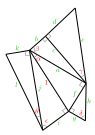
\includegraphics[width = 0.4\textwidth]{lots_of_triangles}
}
\end{tabular}




\section{Right triangle trigonometry examples}


\subsection*{Measuring heights part 1}

\begin{tabular}{cc}
\parbox{0.6\textwidth}{
Given a wall of unknown height \(y\), height \(y\) can be determined by standing a distance \(d\) from the wall and measuring the elevation \(\theta\) of the wall's summit as being viewed from the ground. {\bf \(d\) and \(\theta\) are the only quantities known ahead of any computations.} The adjacent \(d\) is known and the opposite \(y\) is sought, so \(y = d \cdot \tan\theta\). \\
If \(d = 5.6\text{m}\) and \(\theta = 80^\circ\), then the wall's height is \(y = (5.6\text{m})\tan(80^\circ) \approx 31.7592\text{m}\)
} & \parbox{0.3\textwidth}{
\includegraphics[width = 0.3\textwidth]{wall_height_v2}
}
\end{tabular}



\subsection*{Measuring heights part 2}

\begin{tabular}{cc}
\parbox{0.5\textwidth}{
In the image to the right, the height \(y\) of a house is sought. It is generally not possible to measure the height directly, nor is it possible to directly measure the distance between a point underneath the highest point, and a point that has a direct view of the highest point. In this case a rope of known length \(L\) is attached to the top of the house, and pulled taut to a point that has a direct line of sight of the top of the house. The angle \(\theta\) that this rope makes with the ground is measured. {\bf \(L\) and \(\theta\) are the only quantities known ahead of any computations.}
} & \parbox{0.5\textwidth}{
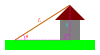
\includegraphics[width = 0.5\textwidth]{house_height}
}
\end{tabular}

The hypotenuse \(L\) of the right triangle is known, and the opposite \(y\) is sought. Therefore: 
\[y = L\sin\theta\]

If \(L = 18.00\text{m}\) and \(\theta = 35^\circ\), then \(y = (18.00\text{m})\sin 35^\circ \approx 10.3244\text{m}\)




\subsection*{Shadows part 1}

\begin{tabular}{cc}
\parbox{0.5\textwidth}{
In the image to the right, an angled roof with a length of \(L\) and incline angle \(\theta\) is given. The assumption being made here is that the sun's rays are completely vertical and parallel. The shadow width \(w\) projected by the roof is sought. {\bf \(L\) and \(\theta\) are the only quantities known ahead of any computations.} Since the hypotenuse \(L\) is known and the adjacent \(w\) is sought, 
\[w = L\cos\theta\]
If \(L = 2.000\text{m}\) and \(\theta = 10^\circ\), then \\ \(w = (2.000\text{m})\cos 10^\circ \approx 1.96962\text{m}\)
} & \parbox{0.5\textwidth}{
\includegraphics[width = 0.5\textwidth]{angled_roof_1}
} 
\end{tabular}



\subsection*{Shadows part 2}

\begin{tabular}{cc}
\parbox{0.5\textwidth}{
In the image to the right, an angled roof with an unknown length of \(L\) and a known incline angle \(\theta\) is shown. The assumption being made here is that the sun's rays are completely vertical and parallel. Making a measurement \(w\) of the shadow width, the length \(L\) of the roof will be computed. {\bf \(w\) and \(\theta\) are the only quantities known ahead of any computations.} Since the adjacent \(w\) is known and the hypotenuse \(L\) is sought, 
\[L = w\sec\theta\] 
If \(w = 5.000\text{m}\) and \(\theta = 15^\circ\), then \\ \(L = (5.000\text{m})\sec 15^\circ \approx 5.17638\text{m}\)
} & \parbox{0.5\textwidth}{
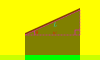
\includegraphics[width = 0.5\textwidth]{angled_roof_2}
}
\end{tabular}




\subsection*{Bridge building part 1}
\begin{tabular}{cc}
\parbox{0.5\textwidth}{
In the image to the right a bridge of unknown length \(L\) is erected to span a river of known width \(w\). The banks are not at equal elevations, so the angle that the bridge makes with a vertical direction is \(\phi\). {\bf \(w\) and \(\phi\) are the only quantities known ahead of any computations.} Since the opposite \(w\) is known, while hypotenuse is sought, 
\[L = w\csc\phi\] 
If \(w = 3.500\text{m}\) and \(\phi = 67^\circ\), then \\ \(L = (3.500\text{m})\csc 67^\circ \approx 3.80226\text{m}\)
} & \parbox{0.5\textwidth}{
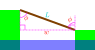
\includegraphics[width = 0.5\textwidth]{bridge_building}
}
\end{tabular}



\subsection*{Shadows part 3}

\begin{tabular}{cc}
\parbox{0.5\textwidth}{
In the image to the right, an angled roof with a length of \(L\) and incline angle \(\theta\) is shown. The sun's rays are parallel and now make an angle of \(\phi\) with the vertical direction. The shadow width \(w\) projected by the roof is sought.  {\bf \(L\), \(\theta\), and \(\phi\) are the only quantities known ahead of any computations.} As seen in the image, the shadow consists of two parts: \(x_1\) is the shadow cast by the horizontal component of the roof, while \(x_2\) is the shadow cast by the vertical component of the roof. 
} & \parbox{0.5\textwidth}{
\includegraphics[width = 0.5\textwidth]{angled_roof_3}
}
\end{tabular}
The horizontal component of the roof is \(x_1 = L\cos\theta\). The vertical component of the roof is \(y_1 = L\sin\theta\). The shadow cast by the horizontal component is simply \(x_1\), while the shadow cast by the vertical component is \(x_2 = y_1\tan\phi = L\sin\theta\tan\phi\). The shadow's width is: 
\[w = x_1 + x_2 = L\cos\theta + L\sin\theta\tan\phi = L(\cos\theta + \sin\theta\tan\phi)\]
If \(L = 2.000\text{m}\), \(\theta = 10^\circ\), and \(\phi = 20^\circ\), then \\ \(w = (2.000\text{m})(\cos 10^\circ + (\sin 10^\circ)(\tan 20^\circ)) \approx 2.09602\text{m}\)



\subsection*{Shadows part 4}

\begin{tabular}{cc}
\parbox{0.5\textwidth}{
In the image to the right, an angled roof with an unknown length of \(L\) and a known incline angle \(\theta\) is shown. The sun's rays are parallel and now make an angle of \(\phi\) with the vertical direction. The shadow width \(w\) is measured, and the unknown roof length \(L\) is sought.  {\bf \(w\), \(\theta\), and \(\phi\) are the only quantities known ahead of any computations.} As seen in the image, the shadow consists of two parts: \(x_1\) is the shadow cast by the horizontal component of the roof, while \(x_2\) is the shadow cast by the vertical component of the roof. 
} & \parbox{0.5\textwidth}{
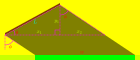
\includegraphics[width = 0.5\textwidth]{angled_roof_4}
}
\end{tabular}
Treating \(L\) as an unknown, the horizontal component of the roof is \(x_1 = L\cos\theta\), and the vertical component of the roof is \(y_1 = L\sin\theta\). The shadow cast by the horizontal component is simply \(x_1\), while the shadow cast by the vertical component is \(x_2 = y_1\tan\phi = L\sin\theta\tan\phi\). The shadow's width is \(w = x_1 + x_2\). Therefore:
\begin{align*}
& w = x_1 + x_2 
\iff w = L\cos\theta + L\sin\theta\tan\phi 
\iff (\cos\theta + \sin\theta \tan\phi)L = w 
\iff L = \frac{w}{\cos\theta + \sin\theta \tan\phi}
\end{align*} 
If \(w = 10.00\text{m}\), \(\theta = 10^\circ\), and \(\phi = 20^\circ\), then \\ \(L = \frac{10.00\text{m}}{\cos 10^\circ + (\sin 10^\circ)(\tan 20^\circ)} \approx 9.54189\text{m}\)



\subsection*{The width of gorges}

\begin{tabular}{cc}
\parbox{0.5\textwidth}{
In the image to the right, the horizontal width of the shown gorge \(w\) is sought. To measure the width of the gorge, the only equipment available is: 
\begin{itemize}
\item A grappling hook with an eye bolt through which a length of rope of known length \(L\) is threaded. 
\item A protractor that can measure the angles between two lines that are physically present. The intersection must be accessible. 
\end{itemize}
What is not available are any other measurements of length, nor telescopes for measuring the angles between lines of sight.
} & \parbox{0.5\textwidth}{
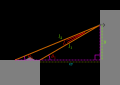
\includegraphics[width = 0.5\textwidth]{gorge_width_2}
}
\end{tabular}

To determine the gorge width, the grappling hook, while threaded onto the rope, is launched and embedded into the far wall. One end of the rope is secured to the edge of the gorge, while the rope is pulled taut and the other end secured further away from the gorge so that the rope remains taut. The angles the rope makes with the horizontal surface are measured: \(\theta_1\) is the angle at the edge of the gorge, while \(\theta_2\) is the angle at the other end. {\bf The quantities \(L\), \(\theta_1\), and \(\theta_2\) are the only quantities that are known ahead of any computations.}

There are two right triangles present. From the common opposite of \(y\), the lengths of each rope segment are \(l_1 = y\csc\theta_1\) and \(l_2 = y\csc\theta_2\). The total length of rope is \(L = l_1 + l_2\), so therefore:
\begin{align*}
& L = l_1 + l_2 
\iff y\csc\theta_1 + y\csc\theta_2 = L 
\iff (\csc\theta_1 + \csc\theta_2)y = L 
\iff y = \frac{L}{\csc\theta_1 + \csc\theta_2}
\end{align*}

Now it is easily seen that \(w = y\cot\theta_1 = \frac{L\cot\theta_1}{\csc\theta_1 + \csc\theta_2}\). Therefore:
\[w = \frac{L\cot\theta_1}{\csc\theta_1 + \csc\theta_2}\]

If \(L = 100\text{m} = 1.000 \times 10^2 \;\text{m}\), \(\theta_1 = 25^\circ\), and \(\theta_2 = 20^\circ\), then \(w = \frac{(1.000 \times 10^2 \;\text{m})\cot 25^\circ}{\csc 25^\circ + \csc 20^\circ} \approx 4.05388 \times 10^1 \;\text{m} = 40.5388\text{m}\)

\vspace{5mm}

\textbf{another approach:}

There are many different approaches to solving the previous problem. The width \(w\) is the sought after value, so another approach is to build a equation that involves \(w\), as opposed to first solving for \(y\). Treating \(w\) as an unknown, \(l_1 = w\sec\theta_1\), and \(y = w\tan\theta_1\), and \(l_2 = y\csc\theta_2 = w\tan\theta_1\csc\theta_2\) so 
\begin{align*}
& l_1 + l_2 = L 
\iff w\sec\theta_1 + w\tan\theta_1\csc\theta_2 = L 
\iff (\sec\theta_1 + \tan\theta_1\csc\theta_2)w = L \\
\iff & w = \frac{L}{\sec\theta_1 + \tan\theta_1\csc\theta_2}
\end{align*} 

Dividing the top and bottom of the quotient by \(\tan\theta_1\) gives \(w = \frac{L/\tan\theta_1}{\sec\theta_1/\tan\theta_1 + \csc\theta_2} = \frac{L\cot\theta_1}{\csc\theta_1 + \csc\theta_2}\) which is equivalent to the expression for \(w\) derived by the original approach.

At this point, a mention should be made that expressions can become complex very rapidly. If the symbols \(L\), \(\theta_1\), and \(\theta_2\) had been replaced with their actual values, this complexity would not exist. Replacing \(L\), \(\theta_1\), and \(\theta_2\) with their assigned values however eliminates the generality of the final solution. In addition, arithmetic using the real values of \(L\), \(\theta_1\), and \(\theta_2\) will slowly, but inevitably, generate round off error. To tame the complexity, while still retaining generality, additional symbols can be utilized to shorthand more complicated expressions. For example, in the equation \(w\sec\theta_1 + w\tan\theta_1\csc\theta_2 = L\), the relatively complicated coefficient of \(\tan\theta_1\csc\theta_2\) can be abbreviated by defining \(a = \tan\theta_1\csc\theta_2\). With these abbreviations, the equation is now \(w \cdot \sec\theta_1 + w \cdot a = L \iff (\sec\theta_1 + a)w = L \iff w = \frac{L}{\sec\theta_1 + a}\). Therefore we can conclude that 
\[w = \frac{L}{\sec\theta_1 + a}  \quad \text{where} \quad a = \tan\theta_1\csc\theta_2\] 

If the same values for \(L\), \(\theta_1\), and \(\theta_2\) are used: \(L = 100\text{m} = 1.000 \times 10^2 \;\text{m}\), \(\theta_1 = 25^\circ\), and \(\theta_2 = 20^\circ\), then \(a \approx 1.36339\), and \(w \approx 4.05389 \times 10^1 \;\text{m} = 40.5389\text{m}\). The small difference from the previously computed \(w\) in the last decimal position is thanks to round off error. If the value of \(a\) were stored in your calculator's memory to a much higher precision, this problem would be greatly diminished. 




\subsection*{The height of mountains part 1}

\begin{tabular}{cc}
\parbox{0.5\textwidth}{
Given a mountain with height \(y\), the distance to a ground level point directly beneath the summit cannot be measured directly, as the ground level point beneath the summit is often physically inaccessible within the bulk of the mountain. To measure the mountain's height, two vantage points separated by a known distance of \(d\) are chosen where the second vantage point is directly in between the first vantage point and the ground level point beneath the summit. \(\theta_1\) and \(\theta_2\) are the line of sight elevations of the summit from the first and second vantage points respectively. {\bf Only \(d\), \(\theta_1\), and \(\theta_2\) are measured and known ahead of any computations}. 
} & \parbox{0.5\textwidth}{
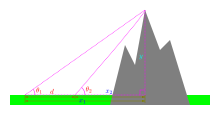
\includegraphics[width = 0.5\textwidth]{mountain_height_v2}
}
\end{tabular}
\(x_1\) and \(x_2\) are the horizontal distances from mountain summit of the first and second vantage points respectively. The two right triangles have opposites of \(y\) and adjacents of \(x_1\) and \(x_2\)  respectively, so computing \(x_1\) and \(x_2\) while treating \(y\) as an unknown gives \(x_1 = y\cot\theta_1\) and \(x_2 = y\cot\theta_2\). \(d = x_1 - x_2\) so: 
\begin{align*}
& d = x_1 - x_2 
\iff d = y\cot\theta_1 - y\cot\theta_2 
\iff (\cot\theta_1 - \cot\theta_2)y = d 
\iff y = \frac{d}{\cot\theta_1 - \cot\theta_2}
\end{align*}
Therefore \(y = \frac{d}{\cot\theta_1 - \cot\theta_2}\) computes the mountain's height given the ground level, accessible, measurements of \(d\), \(\theta_1\), and \(\theta_2\). As an example, given \(d = 96.0210\text{m}\), \(\theta_1 = 70^\circ\), and \(\theta_2 = 75^\circ\), then \(y = \frac{96.02\text{m}}{\cot(70^\circ) - \cot(75^\circ)} \approx 1.00000 \times 10^3\text{m} = 1.00000\text{km}\).

\vspace{5mm}

\textbf{another approach:}

There are many different approaches to solving the previous problem. For example, if we had instead treated \(x_1\) as an unknown, we can compute \(y = x_1\tan\theta_1\) and then \(x_2 = y\cot\theta_2 = x_1 \cdot \tan\theta_1 \cdot \cot\theta_2\) so the condition \(d = x_1 - x_2\) becomes: 
\begin{align*}
& d = x_1 - x_2 
\iff d = x_1 - x_1 \cdot \tan\theta_1 \cdot \cot\theta_2 
\iff (1 - \tan\theta_1 \cdot \cot\theta_2)x_1 = d 
\iff x_1 = \frac{d}{1 - \tan\theta_1 \cdot \cot\theta_2} 
\end{align*}
Now with the value of \(x_1\), 
\[y = x_1\tan\theta_1 = \frac{d\tan\theta_1}{1 - \tan\theta_1 \cdot \cot\theta_2} = \frac{d}{\cot\theta_1 - \cot\theta_2}\]

\vspace{5mm}

\textbf{another approach:}

If we had instead treated \(x_2\) as an unknown, we can compute \(y = x_2\tan\theta_2\) and then \(x_1 = y\cot\theta_1 = x_2 \cdot \tan\theta_2 \cdot \cot\theta_1\) so the condition \(d = x_1 - x_2\) becomes: 
\begin{align*}
& d = x_1 - x_2 
\iff d = x_2 \cdot \tan\theta_2 \cdot \cot\theta_1 - x_2
\iff (\tan\theta_2 \cdot \cot\theta_1 - 1)x_2 = d 
\iff x_2 = \frac{d}{\tan\theta_2 \cdot \cot\theta_1 - 1} 
\end{align*}
Now with the value of \(x_2\), 
\[y = x_2\tan\theta_2 = \frac{d\tan\theta_2}{\tan\theta_2 \cdot \cot\theta_1 - 1} = \frac{d}{\cot\theta_1 - \cot\theta_2}\]

\vspace{5mm}

\textbf{another approach:}

We do not have to use \(d = x_1 - x_2\) as the equation that brings everything together. Treating \(x_1\) as an unknown, \(d = x_1 - x_2\) gives \(x_2 = x_1 - d\). The height \(y\) is both \(y = x_1\tan\theta_1\) and \(y = x_2\tan\theta_2 = (x_1 - d)\tan\theta_2\). Since both expressions for \(y\) must be equal, 
\begin{align*}
& x_1\tan\theta_1 = (x_1 - d)\tan\theta_2 
\iff x_1\tan\theta_1 = x_1\tan\theta_2 - d\tan\theta_2 
\iff x_1\tan\theta_2 - x_1\tan\theta_1 = d\tan\theta_2 \\
\iff & (\tan\theta_2 - \tan\theta_1)x_1 = d\tan\theta_2 
\iff x_1 = \frac{d\tan\theta_2}{\tan\theta_2 - \tan\theta_1}
\end{align*}  
Now with the value of \(x_1\), 
\[y = x_1\tan\theta_1 = \frac{d \tan\theta_1 \tan\theta_2}{\tan\theta_2 - \tan\theta_1} = \frac{d}{\cot\theta_1 - \cot\theta_2}\]




\subsection*{The height of mountains part 2}

\begin{tabular}{cc}
\parbox{0.5\textwidth}{
In the image to the right, the height \(y\) of a mountain is being measured by recording the line-of-sight elevation angle of the summit at two vantage points. The \(1^\text{st}\) vantage point is on the top of an incline that faces the hill, while the \(2^\text{nd}\) vantage point is at the bottom of the same incline, at the elevation from which the mountain's height will be measured. The angle of elevation from the \(1^\text{st}\) vantage point is \(\theta_1\), while the angle of elevation from the \(2^\text{nd}\) vantage point is \(\theta_2\). It is also known that the vantage points are separated by a distance of \(d\), and that the angle of the incline is \(\phi\). {\bf The quantities \(d\), \(\phi\), \(\theta_1\), and \(\theta_2\) are the only quantities that are known ahead of any computations.}
} & \parbox{0.5\textwidth}{
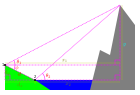
\includegraphics[width = 0.5\textwidth]{mountain_height_2}
}
\end{tabular}

The horizontal displacement that separates the two vantage points is \(d_x = d\cos\phi\). The vertical displacement that separates the two vantage points is \(d_y = d\sin\phi\). The elevation of the peak above vantage point 1 is \(y - d_y\). The \emph{horizontal} distance of vantage point 1 from the summit is \(x_1 = (y - d_y)\cot\theta_1\). The \emph{horizontal} distance of vantage point 2 from the summit is \(x_2 = y\cot\theta_2\). The difference between these horizontal distances is the horizontal displacement that separates the two vantage points: \(x_1 - x_2 = d_x\). Therefore:
\begin{align*}
& x_1 - x_2 = d_x 
\iff (y - d_y)\cot\theta_1 - y\cot\theta_2 = d_x 
\iff (y\cot\theta_1 - d_y\cot\theta_1) - y\cot\theta_2 = d_x \\
\iff & y(\cot\theta_1 - \cot\theta_2) = d_x + d_y\cot\theta_1 
\iff y = \frac{d_x + d_y\cot\theta_1}{\cot\theta_1 - \cot\theta_2}
\end{align*}

Therefore: 
\[y = \frac{d_x + d_y\cot\theta_1}{\cot\theta_1 - \cot\theta_2} \quad \text{where} \quad d_x = d\cos\phi \quad \text{and} \quad d_y = d\sin\phi\]

If \(d = 100\text{m} = 1.000 \times 10^2 \;\text{m}\), \(\phi = 30^\circ\), \(\theta_1 = 39^\circ\), and \(\theta_2 = 40^\circ\), then \\
\(d_x \approx 8.66025 \times 10^1 \;\text{m}\), \(d_y = 5.00000 \times 10^1 \;\text{m}\), and 
\[y \approx \frac{(8.66025 \times 10^1 \;\text{m}) + (5.00000 \times 10^1 \;\text{m})\cot(39^\circ)}{\cot(39^\circ) - \cot(40^\circ)} \approx 3.43846 \times 10^3 \;\text{m} = 3.43846\text{km}\]




%\pagebreak

\subsection*{Bridge building part 2}

\begin{tabular}{cc}
\parbox{0.5\textwidth}{
In the image to the right a bridge of unknown length \(L\) is erected to span a river. The banks are not at equal elevations, so the angle that the bridge makes with a vertical direction is \(\phi\). This time, the river's width is {\bf not} known in advance. A vertical post of known height \(d\) is erected on the upper bank, and a suspension cable connects the top of the post to the lower end of the bridge. The suspension cable makes an angle of \(\theta\) with the deck of the bridge.  {\bf \(d\), \(\phi\), and \(\theta\) are the only quantities known ahead of any computations.} 
} & \parbox{0.5\textwidth}{
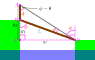
\includegraphics[width = 0.5\textwidth]{bridge_building_2}
}
\end{tabular}
To aid in the discussion to follow, 4 points have been labeled. Point \(A\) is the top of the post; point \(B\) is the raised end of the bridge; point \(C\) is the point directly beneath the raised end of the bridge, at the same elevation as the lower end of the bridge; and point \(D\) is the lower end of the bridge. The two right triangles formed are triangle \(\Delta_1\) with vertices \(B\), \(C\), and \(D\), and triangle \(\Delta_2\) with vertices \(A\), \(C\), and \(D\). The named angle of \(\Delta_1\) will be at point \(B\) and is simply \(\phi\). The named angle of \(\Delta_2\) will be at point \(A\). Since the suspension cable makes an angle of \(\phi - \theta\) to the vertical, the angle of \(\Delta_2\) at point \(A\) is \(\phi - \theta\). 

Both triangles have the river width \(w\) as their opposite. The difference between the adjacent \(y_2\) of triangle \(\Delta_2\) and the adjacent \(y_1\) of triangle \(\Delta_1\) is the height of the post \(d\). To exploit this fact, treating \(w\) as an unknown, the adjacent of \(\Delta_1\) is \(y_1 = w\cot\phi\), and the adjacent of \(\Delta_2\) is \(y_2 = w\cot(\phi - \theta)\). The difference is \(y_2 - y_1 = w\cot(\phi - \theta) - w\cot\phi\) which should equal \(d\) so therefore:
\begin{align*}
& y_2 - y_1 = d 
\iff w\cot(\phi - \theta) - w\cot\phi = d
\iff w(\cot(\phi - \theta) - \cot\phi) = d 
\iff w = \frac{d}{\cot(\phi - \theta) - \cot\phi}
\end{align*}

Now we know the river's width \(w = \frac{d}{\cot(\phi - \theta) - \cot\phi}\). The bridge's length is the hypotenuse of \(\Delta_1\) and is 
\[L = w\csc\phi = \frac{d\csc\phi}{\cot(\phi - \theta) - \cot\phi}\]

If \(d = 2.000\text{m}\), \(\phi = 85^\circ\), and \(\theta = 10^\circ\), then \(L = \frac{(2.000\text{m})\csc 85^\circ}{\cot 75^\circ - \cot 85^\circ} \approx 11.1251\text{m}\)



\pagebreak

\subsection*{Bridge building part 3}

\begin{tabular}{cc}
\parbox{0.5\textwidth}{
In the image to the right a bridge of unknown length \(L\) is erected to span a river. The banks are not at equal elevations, so the angle that the bridge makes with a vertical direction is \(\phi\). This time, the river's width is {\bf not} known in advance. A vertical post of known height \(d\) is erected on the lower bank, and a suspension cable connects the top of the post to the upper end of the bridge. The suspension cable makes an angle of \(\theta\) with the deck of the bridge.  {\bf \(d\), \(\phi\), and \(\theta\) are the only quantities known ahead of any computations.} 
} & \parbox{0.5\textwidth}{
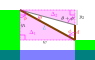
\includegraphics[width = 0.5\textwidth]{bridge_building_3}
}
\end{tabular}
To aid in the discussion to follow, 2 right triangles are highlighted in the image. Triangle \(\Delta_1\) has the bridge as its hypotenuse, while triangle \(\Delta_2\) has the suspension cable as its hypotenuse. The named angle of \(\Delta_1\) is the angle that the bridge makes with the vertical direction, namely \(\phi\). The named angle of \(\Delta_2\) is the angle that the suspension cable makes with the vertical direction, namely \(\phi + \theta\). 

Both triangles have the river width \(w\) as their opposite. The difference between the adjacent \(y_1\) of triangle \(\Delta_1\) and the adjacent \(y_2\) of triangle \(\Delta_2\) is the height of the post \(d\). To exploit this fact, treating \(w\) as an unknown, the adjacent of \(\Delta_1\) is \(y_1 = w\cot\phi\), and the adjacent of \(\Delta_2\) is \(y_2 = w\cot(\phi + \theta)\). The difference is \(y_1 - y_2 = w\cot\phi - w\cot(\phi + \theta)\) which should equal \(d\) so therefore:
\begin{align*}
& y_1 - y_2 = d 
\iff w\cot\phi - w\cot(\phi + \theta) = d
\iff w(\cot\phi - \cot(\phi + \theta)) = d 
\iff w = \frac{d}{\cot\phi - \cot(\phi + \theta)}
\end{align*}

Now we know the river's width \(w = \frac{d}{\cot\phi - \cot(\phi + \theta)}\). The bridge's length is the hypotenuse of \(\Delta_1\) and is 
\[L = w\csc\phi = \frac{d\csc\phi}{\cot\phi - \cot(\phi + \theta)}\]

If \(d = 2.000\text{m}\), \(\phi = 75^\circ\), and \(\theta = 10^\circ\), then \(L = \frac{(2.000\text{m})\csc 75^\circ}{\cot 75^\circ - \cot 85^\circ} \approx 11.4737\text{m}\)



\section{Inverse Trigonometric Functions}


\parbox{0.5\textwidth}{
\includegraphics[scale = 0.5]{arccos_and_arcsin.png} \\
dark red \(= \arccos\theta\); ~~~ light red \(= \arcsin\theta\)
} 

\parbox{0.5\textwidth}{
\includegraphics[scale = 0.3]{arctan.png} \\
dark green \(= \arctan\theta\)
} 




\end{document}




